\chapter{روش پیشنهادی}
\clearpage

در این فصل، به تشریح کامل روش پیشنهادی می‌پردازیم. نخست، به‌عنوان پیش‌نیاز، به تعریف تبدیل موجک\LTRfootnote{Wavelet Transform} و
اسکالوگرام\LTRfootnote{Scalogram}
خواهیم پرداخت. سپس، روش پایه و معماری آن را به تفصیل مورد بررسی قرار می‌دهیم. در نهایت، با تحلیل این معماری، زمینه‌های مستعد بهبود در آن شناسایی شده و سپس نوآوری‌های ارائه شده در این پژوهش که برای رفع این چالش‌ها طراحی شده‌اند، به تفصیل تشریح خواهند شد.

\section{تبدیل موجک}

تبدیل موجک یکی از ابزارهای قدرتمند در پردازش سیگنال است که برای تحلیل سیگنال‌ها در هر دو حوزه‌ی زمان و فرکانس به صورت همزمان به کار می‌رود. این ویژگی، تبدیل موجک را از ابزارهای کلاسیک مانند
تبدیل فوریه\LTRfootnote{Fourier Transform}
متمایز می‌سازد. تبدیل فوریه، سیگنال را به مولفه‌های فرکانسی تشکیل‌دهنده‌ی آن از طریق دو طیف دامنه و فاز تجزیه می‌کند. طیف دامنه نشان می‌دهد که هر مولفه‌ی فرکانسی با چه شدتی در کل سیگنال حضور دارد، اما اطلاعاتی در مورد زمان وقوع آن ارائه نمی‌دهد. اگرچه طیف فاز به صورت غیرمستقیم حاوی اطلاعات زمانی است، اما تفسیر آن برای محلی‌سازی رویدادها در زمان بسیار دشوار و غیرمستقیم است. به عبارت دیگر، تبدیل فوریه در نمایش همزمان رویدادها در حوزه‌ی زمان و فرکانس دارای محدودیت است. در مقابل، تبدیل موجک با استفاده از توابعی به نام
موجک مادر\LTRfootnote{Mother Wavelet}
که در زمان و فرکانس محدود هستند، این محدودیت را برطرف می‌سازد.

ایده‌ی اصلی در تبدیل موجک، مقایسه‌ی سیگنال با نسخه‌های جابه‌جا شده و مقیاس‌گذاری شده از یک موجک مادر است. جابه‌جایی به منظور محلی‌سازی تحلیل در زمان و مقیاس‌گذاری به منظور محلی‌سازی تحلیل در فرکانس انجام می‌شود. مقیاس‌های کوچک (فشرده‌سازی موجک) متناظر با فرکانس‌های بالا و مقیاس‌های بزرگ (کشیده‌سازی موجک) متناظر با فرکانس‌های پایین هستند.

تبدیل موجک به دو دسته‌ی اصلی گسسته (\lr{DWT\LTRfootnote{Discrete Wavelet Transform}}
و پیوسته (\lr{CWT\LTRfootnote{Continuous Wavelet Transform}})
تقسیم می‌شوند که در این پژوهش از تبدیل موجک پیوسته استفاده کرده‌ایم.

تبدیل موجک یک سیگنال زمانی $x(t)$
به فرم زیر تعریف می‌گردد:
\begin{equation}
    \label{eq:wavelet-transform}
    CWT(a, b) = \int_{-\infty}^{\infty} x(t) \psi_{a,b}(t) dt
\end{equation}
که در این معادله، $\psi_{a,b}(t)$
موجک دختر\LTRfootnote{Daughter Wavelet}
نامیده می‌شود که نسخه‌ی مقیاس‌گذاری و جابه‌جا شده است و به فرم زیر تعریف می‌گردد:
\begin{equation}
    \label{eq:daughter-wavelet}
    \psi_{a,b}(t) = \frac{1}{\sqrt{|a|}} \psi \left( \frac{t - b}{a} \right)
\end{equation}
در این رابطه، پارامتر $a$ مقیاس است
که با فرکانس رابطه‌ی معکوس دارد. پارامتر $b$
بیانگر میزان جابه‌جایی در محور زمان است و ضریب
$\frac{1}{\sqrt{|a|}}$
برای نرمال‌سازی انرژی موجک به‌کار می‌رود.
$\psi(t)$
نیز یک تابع ریاضی است که باید دارای میانگین صفر و انرژی محدود در تمام دامنه باشد. برای مثال موجک مورلت\LTRfootnote{Morlet Wavelet}
که فرمول آن به فرم رابطه‌ی \ref{eq:morlet-wavelet}
می‌باشد، یک موجک بسیار کاربردی در حوزه‌ی سیگنال‌های دنیای واقعی، به‌خصوص سیگنال‌های مربوط به فعالیت انسان می‌باشد. چرا که در این سیگنال‌ها، معمولا نوسانات و فرکانس‌های غیر ایستا داریم که به سرعت محو می‌شوند و موجک مورلت به‌دلیل دارا بودن $e^{\frac{-t^2}{2}}$
که به آن اثر محوشدگی را می‌دهد، برای این‌گونه سیگنال‌ها بسیار مناسب است.
\begin{equation}
    \label{eq:morlet-wavelet}
    \psi(t) = \frac{\cos(\omega_0 t) e^{-\frac{t^2}{2}}}{\pi^{\frac{1}{4}}}
\end{equation}
خروجی \lr{CWT}
مجموعه‌ای از ضرایب است که میزان شباهت سیگنال $x(t)$
را با موجک با مقیاس $a$ و زمان $b$
نشان می‌دهد. این ضرایب یک نمایش دوبعدی از سیگنال یک بعدی اولیه ارائه می‌دهند که به آن اسکالوگرام می‌گویند. در یک اسکالوگرام محور افقی بیانگر میزان جابه‌جایی یا همان $b$ و
محور عمودی بیانگر مقیاس‌ها می‌باشد. یک نمونه اسکالوگرام در شکل \ref{fig:wavelet-plot} قابل مشاهده می‌باشد.
\begin{figure}[htb!]
\centering
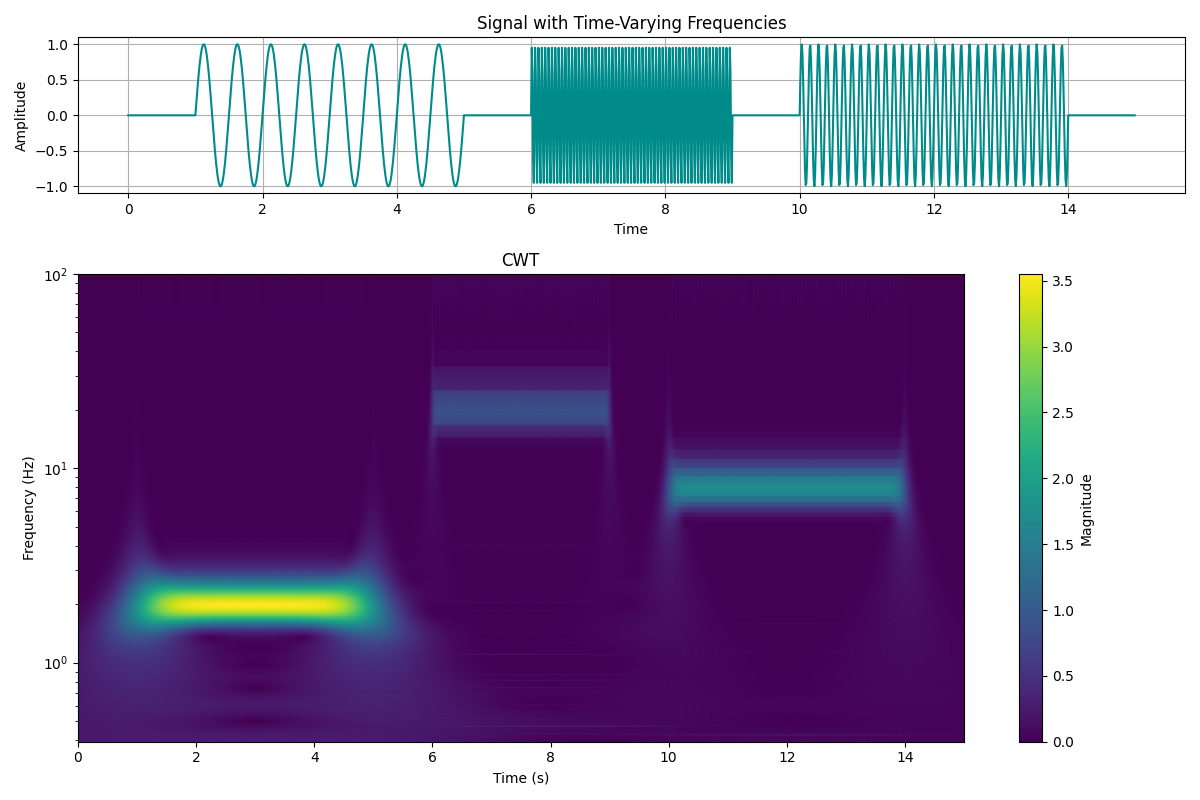
\includegraphics[width=1\textwidth]{Images/Chapter3/wavelet-plot.png}
\caption{نمونه اسکالوگرام برای یک موج متغیر در زمان}
\label{fig:wavelet-plot}
\end{figure}

\section{روش پایه}

معماری کلی پیش‌آموزش خودنظارتی روش پیشنهادی در شکل \ref{fig:proposed-method-pretraining}
قابل مشاهده است. این معماری توسط طاقانکی و همکاران\cite{taghanaki2023self}
برای پیش‌آموزش یک مدل جهت استخراج بازنمایی‌های مفید از روی داده‌های سیگنال مربوط به شناسایی فعالیت انسان ارائه شد. این معماری با این فرضیه طراحی شده است که اطلاعات مفید مربوط به فعالیت در هر دو حوزه زمان و فرکانس نهفته است. به همین منظور، از دو مسیر پردازشی مجزا برای استخراج ویژگی از سیگنال ورودی استفاده می‌شود. یک کدگذار سیگنال که وظیفه‌ی آن پردازش داده‌های خام سیگنال می‌باشد و یک کدگذار اسکالوگرام که وظیفه‌ی آن پردازش اسکالوگرام‌های حاصل از تبدیل موجک
بر روی داده‌های خام سیگنال می‌باشد.

\begin{figure}[ht]
\centering
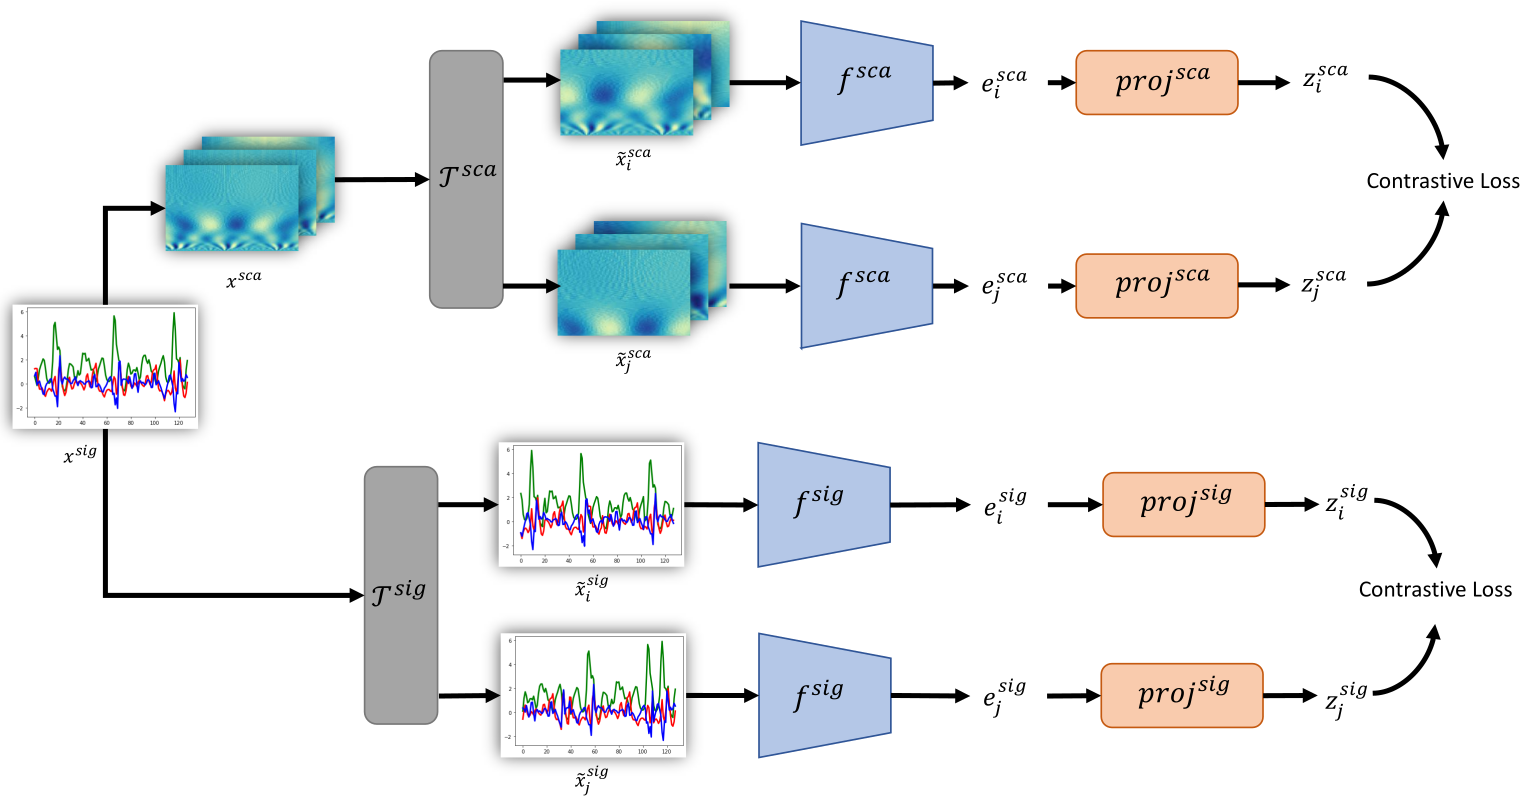
\includegraphics[width=1\textwidth]{Images/Chapter3/proposed-method-pretraining.png}
\caption{معماری کلی پیش‌آموزش در روش پیشنهادی}
\label{fig:proposed-method-pretraining}
\end{figure}

در ادامه به بررسی جزئیات مربوط به هر دو مسیر آموزش کدگذار می‌پردازیم.

\subsection{کدگذار سیگنال}

این بخش از معماری وظیفه‌ی یادگیری از روی داده‌های خام سیگنال در حوزه‌ی زمان را بر عهده دارد. برای آموزش این بخش، از چارچوب یادگیری تباینی
\lr{SimCLR}
که در فصل قبل درباره‌ی جزئیات آن توضیح دادیم استفاده شده است. کدگذار سیگنال یا
$\mathcal{H}_{sig}$
از یک شبکه عصبی شامل ۳ لایه پیچشی یک بعدی تشکیل شده است. سپس خروجی $\mathcal{H}_{sig}$
به یک شبکه نگاشت داده می‌شود و در نهایت بر روی خروجی شبکه نگاشت تابع هزینه تباینی \lr{NT-Xent} به‌فرم معادله \ref{eq:simclr-loss}
اعمال می‌شود.
پیاده‌سازی چارچوب \lr{SimCLR} مستلزم تعریف مجموعه‌ای از تبدیلات داده‌افزایی است. در این مسیر، تبدیلات زیر برای اعمال بر روی سیگنال خام زمانی به کار گرفته شده‌اند:
\begin{itemize}
    \item\textbf{نویز:} یک نویز تصادفی گوسی با میانگین صفر و انحراف معیار $0.1$ اعمال می‌شود.
    \item\textbf{مقیاس‌دهی\LTRfootnote{Scale}:}
    یک مقدار تصادفی با میانگین $1$ و انحراف معیار $0.2$ در سیگنال ضرب می‌شود.
    \item\textbf{معکوس‌سازی زمانی\LTRfootnote{Time Flip}:}
    با یک احتمال ثابت، پنجره سیگنال ورودی نسبت به زمان معکوس می‌گردد. ایده‌ی پشت این تبدیل این است که یک فعالیت ممکن است در جهت برعکس انجام شود.
    \item\textbf{بر زدن کانال‌ها\LTRfootnote{Channel Shuffle}:}
    با یک احتمال ثابت، کانال‌های سیگنال ورودی به‌صورت تصادفی با یکدیگر جابه‌جا می‌شوند. ایده‌ی پشت این تبدیل این است که ممکن است حسگر در یک جهتی عمود بر جهت استاندارد قرار گرفته باشد. مثلا جهت قرار گرفتن تلفن همراه هوشمند در جیب شخص. نکته‌ی مهم در رابطه با این تبدیل این است که فقط کانال‌های مربوط به هر دستگاه باید با یکدیگر جابه‌جا شوند. مثلا اگر کانال‌های اول تا سوم برای شتاب‌سنج و کانال‌های چهارم تا ششم برای ژیروسکوپ باشند، کانال‌های اول تا سوم با یکدیگر و کانال‌های چهارم تا ششم نیز با یکدیگر جابه‌جا می‌شوند.
    \item\textbf{جایگشت:} سیگنال ورودی به قطعاتی تقسیم می‌شود و این قطعات با یکدیگر جابه‌جا می‌شوند. ایده‌ی پشت این تبدیل این است که ممکن است ترتیب بخش‌های مربوط به انجام یک فعالیت تغییر کنند.
    \item\textbf{چرخش:}
    سیگنال ورودی حول یک محور تصادفی و به میزان درجه‌ی تصادفی چرخش داده می‌شود. در واقع چرخش، حالت کلی‌تر از بر زدن کانال‌ها می‌باشد.
\end{itemize}

انتخاب تبدیلات بهینه و ترکیب آن‌ها، فرایندی تجربی و وابسته به مشخصات هر مجموعه داده است. اما به‌طور کلی تبدیلات نه باید به‌قدری سخت و شدیدا تصادفی باشند که مدل کلا نتواند الگویی کشف کند، و نه باید به‌قدری ساده باشند که مدل به سراغ کشف بازنمایی‌های مفید و جامع نرود.

\subsection{کدگذار اسکالوگرام}

این بخش از معماری وظیفه‌ی یادگیری از روی اسکالوگرام‌های حاصل از اعمال تبدیل موجک بر روی سیگنال‌ها را بر عهده دارد. همانند کدگذار سیگنال، در کدگذار اسکالوگرام نیز از روش \lr{SimCLR}
برای آموزش مدل استفاده شده است. کدگذار اسکالوگرام یا
$\mathcal{H}_{sca}$
از یک شبکه عصبی شامل ۳ لایه پیچشی دو بعدی تشکیل شده است. قبل از این که یک پنجره‌ی چندکاناله از داده‌ها وارد این شبکه شوند، بر روی آن‌ها تبدیل موجک اعمال می‌شود و با اسکالوگرام حاصل می‌توان مانند یک تصویر رفتار کرد.

روش‌های داده‌افزایی به‌کار رفته در کدگذار اسکالوگرام نیز به شرح زیر می‌باشند:
\begin{itemize}
    \item\textbf{اعوجاج رنگ تصادفی\LTRfootnote{Random Color Distortion}:}
    در این تبدیل، هر کانال مربوط به هر حسگر را یک رنگ در نظر می‌گیریم و رنگ آن را به‌صورت تصادفی دچار اعوجاج و تغییرات می‌کنیم. مثلا شدت رنگ‌ها را افزایش می‌دهیم و یا آن را به فرم سیاه و سفید درمی‌آوریم.
    \item\textbf{برش تصادفی:}
    به‌صورت تصادفی اسکالوگرام‌ها را برش می‌زنیم.
    \item\textbf{معکوس‌سازی زمانی:}
    اسکالوگرام‌ها را به‌صورت افقی معکوس می‌کنیم.
\end{itemize}

\subsection{تنظیم دقیق مدل}

پس از این که هر دو کدگذار فرایند پیش‌آموزش را پشت سر گذاشتند، مانند روش \lr{SimCLR}
شبکه نگاشت کنار گذاشته می‌شود و به‌جای آن یک شبکه متشکل از دو لایه‌ی تماما متصل برای دسته‌بندی قرار داده می‌شوند. این کار را برای هر دو کدگذار به‌صورت مستقل انجام می‌دهیم. سپس وزن‌های لایه‌های پیچشی هر دو کدگذار تثبیت می‌شوند. این عمل دو هدف اصلی را دنبال می‌کند: اولا، از بیش‌برازش مدل بر روی داده‌های برچسب‌دار که معمولا حجم کمتری دارند جلوگیری می‌کند و ثانیا، بازنمایی‌های کلی و مفیدی که در مرحله پیش‌آموزش یاد گرفته شده‌اند، حفظ می‌شوند. در نهایت دو دسته‌بندی کننده خواهیم داشت که هر یک جداگانه آموزش دیده‌اند؛ یکی بر روی داده‌های خام و دیگری بر روی اسکالوگرام‌ها. در نهایت برای به‌دست آمدن دسته‌بند نهایی، بایستی خروجی دو دسته‌بند با یکدیگر ادغام شوند. در این روش، از راهبرد
ادغام در سطح امتیاز\LTRfootnote{Score-Level Fusion}
که به آن
ادغام دیرهنگام\LTRfootnote{Late Fusion}
نیز گفته می‌شود، استفاده شده است. در این روش، بردارهای احتمال خروجی از هر دو دسته‌بند (به عنوان مثال از طریق میانگین‌گیری) با یکدیگر ترکیب شده و سپس دسته‌ی نهایی بر اساس بیشترین امتیاز در بردار حاصل انتخاب می‌گردد.

\section{نوآوری‌های پیشنهادی}

همان‌طور که تشریح شد، روش پایه یک چارچوب قدرتمند و منطقی برای یادگیری بازنمایی از سیگنال‌های فعالیت انسان ارائه می‌دهد. با این وجود، تحلیل دقیق این معماری نشان می‌دهد که چندین مولفه کلیدی در آن، ظرفیت بهبود و بهینه‌سازی را دارا هستند. در این پژوهش، دو حوزه اصلی برای ارتقای مدل پایه شناسایی و مورد هدف قرار گرفته است:
\begin{itemize}
    \item\textbf{الگوریتم یادگیری تباینی:}
    با وجود این که چارچوب یادگیری تباینی \lr{SimCLR}
    عملکرد خوبی از خود در حوزه‌های مختلف نشان داده است، می‌توان از رویکردهای دیگر یادگیری تباینی که در دیگر حوزه‌ها عملکرد بهتری از خود نشان داده‌اند استفاده کرد.
    \item\textbf{راهبرد داده‌افزایی:}
    روش‌های داده‌افزایی اعمال‌شده بر روی اسکالوگرام‌ها مستقیما از حوزه بینایی کامپیوتر اقتباس شده‌اند و ممکن است بهترین گزینه برای داده‌های زمان-فرکانس نباشند. بنابراین، یک راهبرد داده‌افزایی جدید و متناسب با ماهیت این داده‌ها ارائه می‌شود.
\end{itemize}

\subsection{الگوریتم یادگیری تباینی \lr{SwAV}}

الگوریتم یادگیری تباینی
\textbf{تعویض انتساب‌ها میان نماها} یا به‌اختصار \lr{SwAV\LTRfootnote{Swapping Assignments between Views}}،
یک الگوریتم یادگیری تباینی مبتنی بر خوشه‌بندی می‌باشد که توسط کارون و همکاران\cite{caron2020unsupervised} ارائه شد. این الگوریتم با هدف یادگیری بازنمایی‌های بصری قدرتمند بدون نیاز به برچسب‌های انسانی طراحی شده و توانسته است فاصله‌ی عملکردی میان روش‌های خودنظارتی و نظارت‌شده را به شکل چشمگیری کاهش دهد.

ایده‌ی اصلی این الگوریتم بر یک سازوکار پیش‌بینی تعویض‌شده\LTRfootnote{Swapped Prediction}
استوار است. در این روش، به جای مقایسه‌ی مستقیم بردارهای ویژگی حاصل از نماهای مختلف یک تصویر با یکدیگر (کاری که در روش‌های متداولی مانند \lr{SimCLR} انجام می‌شود)، مدل می‌آموزد که تخصیص خوشه‌ی یک نما را از روی بردار ویژگی نمای دیگر پیش‌بینی کند. به عبارت دیگر، اگر دو نمای مختلف از یک تصویر ورودی داشته باشیم، ویژگی‌های استخراج‌شده از نمای اول باید آن‌قدر غنی و معنادار باشند که بتوان با استفاده از آن‌ها، کد خوشه‌ی مربوط به نمای دوم را پیش‌بینی کرد و بالعکس. این فرایند، مدل را وادار می‌سازد تا بازنمایی‌هایی را بیاموزد که نسبت به تبدیلات و تغییرات اعمال‌شده بر روی تصویر (مانند برش، تغییر رنگ و دوران) نامتغیر و پایدار باشند.

\begin{figure}[htb!]
\centering
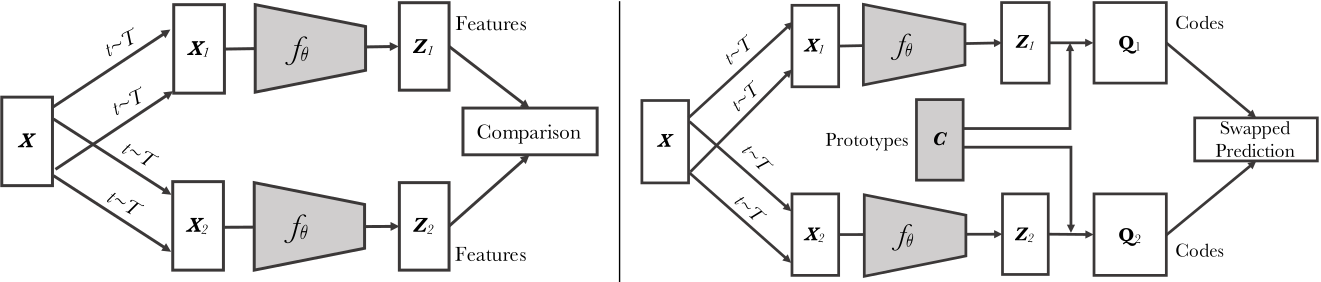
\includegraphics[width=0.8\textwidth]{Images/Chapter3/swav-comparison.png}
\caption{مقایسه‌ی الگوریتم \lr{SwAV} (سمت راست) و \lr{SimCLR} (سمت چپ)}
\label{fig:wavelet-plot}
\end{figure}

یکی از نوآوری‌های کلیدی روش \lr{SwAV}، انجام فرایند خوشه‌بندی به صورت برخط\LTRfootnote{Online}
است. در روش‌های مبتنی بر خوشه‌بندی پیشین
(مانند روش خوشه عمیق\LTRfootnote{Deep Cluster}\cite{caron2018deep})،
فرایند یادگیری به دو مرحله‌ی مجزا و غیر برخط تقسیم می‌شد: ابتدا تمام داده‌ها برای تخصیص به خوشه‌ها پردازش شده و سپس از این تخصیص‌ها به عنوان برچسب‌های کاذب برای آموزش شبکه استفاده می‌شد.  این فرایند نیازمند عبورهای چندباره از کل مجموعه داده بود و مقیاس‌پذیری الگوریتم را با چالش مواجه می‌کرد. اما در \lr{SwAV}، تخصیص خوشه‌ها تنها با استفاده از نمونه‌های موجود در هر دسته‌ی آموزشی از داده‌ها و به صورت آنی انجام می‌شود. این ویژگی باعث می‌شود که \lr{SwAV} بسیار کارآمد بوده و بتواند بر روی مجموعه‌داده‌های بسیار بزرگ نیز به راحتی آموزش ببیند.

\subsubsection{تابع هزینه پیش‌بینی تعویض‌شده}

همان‌طور که اشاره کردیم، هسته‌ی اصلی الگوریتم \lr{SwAV} بر مبنای یک تابع هزینه‌ی منحصربه‌فرد به نام «پیش‌بینی تعویض‌شده» قرار دارد. این تابع هزینه، سازگاری میان نماهای مختلف یک تصویر را نه از طریق مقایسه‌ی مستقیم ویژگی‌ها، بلکه از طریق مقایسه‌ی تخصیص خوشه‌های آن‌ها می‌سنجد.

فرض کنید برای یک تصویر ورودی، دو نمای مختلف با اعمال تبدیلات تصادفی ایجاد کرده‌ایم و پس از عبور آن‌ها از شبکه‌ی کدگذار، بردارهای ویژگی
$z_t$ و $z_s$ را به‌دست آورده‌ایم.
تابع هزینه‌ی \lr{SwAV} برای این زوج ویژگی به صورت زیر تعریف می‌شود:
\begin{equation}
    L(z_t, z_s) = \ell(z_t, q_s) + \ell(z_s, q_t)
    \label{eq:swav-loss}
\end{equation}
در این رابطه:
\begin{itemize}
    \item $z_t$ و $z_s$ بردارهای ویژگی نرمال‌شده‌ی حاصل از دو نما هستند.
    \item $q_t$ و $q_s$ کدهای خوشه یا بردارهای تخصیص نرم\LTRfootnote{Soft Assignment Vectors} مربوط به هر یک از این ویژگی‌ها می‌باشند. این کدها که در عمل یک توزیع احتمال هستند، نشان می‌دهند که هر ویژگی تا چه حد به هر یک از خوشه‌های موجود در مدل تعلق دارد.
    \item $\ell(z,q)$ تابعی است که میزان اختلاف میان یک توزیع پیش‌بینی‌شده (که از $z$ حاصل می‌شود) و یک کد هدف ($q$) را اندازه‌گیری می‌کند.
\end{itemize}
فرمول \ref{eq:swav-loss} دارای دو بخش متقارن است. بخش اول، $\ell(z_t,q_s)$
مدل را وادار می‌کند تا با استفاده از ویژگی نمای اول ($z_t$) کد خوشه‌ی نمای دوم ($q_s$) را پیش‌بینی کند. بخش دوم نیز این فرایند را به‌صورت معکوس انجام می‌دهد. به همین دلیل این سازوکار، پیش‌بینی تعویض‌شده نام گرفته است.

تابع $\ell(z,q)$ در عمل یک تابع هزینه آنتروپی متقاطع است که اختلاف میان دو توزیع احتمال را می‌سنجد:
\begin{itemize}
    \item\textbf{توزیع پیش‌بینی شده \lr{p}:} یک توزیع احتمال که از بردار ویژگی $z$ به دست می‌آید و نشان‌دهنده‌ی پیش‌بینی مدل برای تخصیص آن ویژگی به خوشه‌هاست.
    \item\textbf{کد هدف \lr{q}:} یک توزیع احتمال که به عنوان برچسب نرم عمل می‌کند و از قبل برای نمای دیگر محاسبه شده است.
\end{itemize}

\noindent\textbf{محاسبه توزیع پیش‌بینی‌شده (\lr{p}): از ویژگی به احتمال}

توزیع $p$،
پیش‌بینی مدل از میزان تعلق یک بردار ویژگی $z$
به هر یک از $K$ خوشه موجود را نشان می‌دهد. مراکز خوشه‌ها را با بردارهایی تحت عنوان پیش‌نمونه\LTRfootnote{Prototype} نشان می‌دهیم که این مراکز خوشه‌ها مجموعه‌ای از بردارهای قابل یادگیری $C=\{c_1,...,c_k\}$
در فضای ویژگی هستند.

فرایند تبدیل بردار ویژگی 
$z$
به توزیع احتمال 
$p$
در دو مرحله‌ی اصلی انجام می‌شود: ابتدا محاسبه‌ی امتیازات شباهت و سپس تبدیل این امتیازات به یک توزیع احتمال معتبر.

در گام نخست، مدل میزان شباهت میان بردار ویژگی
$z_t$
و هر یک از 
$K$
بردار مرکز خوشه را محاسبه می‌کند. این شباهت از طریق ضرب داخلی میان بردار ویژگی و هر بردار $c_k$
به دست می‌آید. نتیجه‌ی این عملیات، یک بردار با 
$K$
درایه است که هر درایه‌ی آن، که هر درایه‌ی آن، امتیاز شباهت خام یا \lr{Logit} نامیده می‌شود و نشان‌دهنده‌ی میزان تطابق ویژگی با آن بردار مرکز خوشه خاص است.

امتیازات خام به دست آمده، مقادیری نامحدود هستند و مجموع آن‌ها لزوما برابر با یک نیست. برای تبدیل آن‌ها به یک توزیع احتمال معتبر، از تابع سافت‌مکس\LTRfootnote{Softmax} استفاده می‌شود. این تابع، هر امتیاز را به یک مقدار در بازه‌ی $(0, 1)$ نگاشت کرده و تضمین می‌کند که مجموع تمام احتمالات برابر با یک شود. در این فرایند، از یک پارامتر دما $\tau$ نیز برای کنترل تیزی یا همواری توزیع خروجی استفاده می‌شود. دمای پایین‌تر منجر به توزیعی تیزتر (با قطعیت بیشتر) و دمای بالاتر منجر به توزیعی هموارتر می‌گردد. بنابراین، احتمال تعلق ویژگی 
$z_t$
به خوشه 
$k$ام که با
$p_t^{(k)}$
نمایش داده می‌شود، از طریق فرمول زیر محاسبه می‌گردد:
\begin{equation}
p_t^{(k)} = \frac{\exp(\frac{1}{\tau} z_t^\top c_k)}{\sum_{k'=1}^{K} \exp(\frac{1}{\tau} z_t^\top c_{k'})}
\label{eq:swav-p-calculation}
\end{equation}
در این فرمول،
$z_t^kc_k$
همان ضرب داخلی میان بردار ویژگی و بردار مرکز خوشه $k$ام است.
مخرج کسر نیز مجموع مقادیر صورت کسر برای تمام 
$K$
مرکز خوشه است که برای نرمال‌سازی به کار می‌رود. این توزیع
$p_t$
همان پیش‌بینی مدل برای بردار ویژگی $z_t$ است که در تابع هزینه‌ی آنتروپی متقاطع با کد هدف
$q_s$
مقایسه خواهد شد.

\vspace{0.5em}
\noindent\textbf{محاسبه کدهای هدف \lr{q}: تخصیص بهینه خوشه‌ها}

اکنون به بخش پیچیده‌تر محاسبه‌ی تابع هزینه، یعنی نحوه‌ی تعیین کدهای هدف 
$q$
می‌رسیم. برخلاف توزیع پیش‌بینی‌شده 
$p$
که به سادگی از خروجی شبکه به دست می‌آمد، محاسبه‌ی 
$q$
نیازمند یک سازوکار ویژه برای جلوگیری از یک مشکل اساسی است.

یک چالش مهم در روش‌های مبتنی بر خوشه‌بندی، پدیده‌ای است که با عناوینی چون پاسخ بدیهی\LTRfootnote{Trivial Solution}
یا فروپاشی مدل\LTRfootnote{Model Collapse}
شناخته می‌شود. این مشکل زمانی رخ می‌دهد که مدل یک راه‌حل ساده و بی‌ارزش برای کمینه کردن تابع هزینه پیدا کند. در مسئله‌ی ما، مدل می‌تواند یاد بگیرد که تمام بردارهای ویژگی را به یک خوشه‌ی یکسان تخصیص دهد. در این حالت، اگرچه تابع هزینه به سرعت کمینه می‌شود، اما بازنمایی‌های آموخته‌شده هیچ اطلاعات مفیدی در مورد تمایز میان تصاویر مختلف نخواهند داشت و عملا بی‌ارزش خواهند بود.

برای مقابله با این پدیده، الگوریتم \lr{SwAV}
یک قید افراز برابر\LTRfootnote{Equipartition Constraint}
را بر روی فرایند تخصیص خوشه‌ها اعمال می‌کند. هدف این قید، وادار کردن مدل به استفاده از تمام ظرفیت بردارهای مربوط به مراکز خوشه‌ها است. این قید تضمین می‌کند که نمونه‌های موجود در یک دسته آموزشی از داده‌ها، تا حد امکان به صورت یکنواخت و برابر میان تمام 
$K$
خوشه موجود توزیع شوند.

مسئله‌ی تخصیص بهینه‌ی مجموعه‌ای از منابع (ویژگی‌های مربوط به داده‌ها) به مجموعه‌ای از مقاصد (خوشه‌ها) تحت یک سری قیود، یک مسئله‌ی کلاسیک در ریاضیات و علوم کامپیوتر است که با عنوان مسئله‌ی انتقال بهینه\LTRfootnote{Optimal Transport}
شناخته می‌شود. الگوریتم \lr{SwAV} از این چارچوب قدرتمند ریاضی برای محاسبه‌ی ماتریس تخصیص خوشه‌ها
($Q$) استفاده می‌کند.

برای درک بهتر، می‌توان این مسئله را با یک مثال ملموس توصیف کرد. فرض کنید 
$B$
 انبار (بردارهای ویژگی) و 
$K$
 فروشگاه (خوشه‌ها) داریم. هدف، طراحی یک برنامه‌ی حمل و نقل
 (ماتریس $Q$)
 است که کالاها را از انبارها به فروشگاه‌ها به بهینه‌ترین شکل ممکن ارسال کند. بهینه بودن در اینجا به دو معناست: اولا، مجموع شباهت میان انبارها و فروشگاه‌های متناظرشان بیشینه شود و ثانيا، قیود توزیع عادلانه (قید افراز برابر) که در بخش قبل به آن اشاره شد، رعایت گردد.

 به زبان ریاضی، این مسئله به صورت یافتن ماتریس $Q$ از میان مجموعه‌ی تمام ماتریس‌های معتبر 
$\mathcal{Q}$
(که در قیود افراز برابر صدق می‌کنند) تعریف می‌شود که عبارت زیر را بیشینه کند:
\begin{equation}
\max_{Q \in \mathcal{Q}} Tr(Q^\top C^\top Z) + \epsilon H(Q)
\label{eq:swav-optimal-transport}
\end{equation}
در این رابطه:
\begin{itemize}
    \item عبارت
    $Tr(Q^\top C^\top Z)$،
    مجموع وزن‌دار شباهت‌ها میان تمام ویژگی‌ها و تمام مراکز خوشه‌هاست. هدف اصلی، بیشینه کردن این مقدار است.
    \item عبارت
    $\epsilon H(Q)$،
    یک جمله‌ی تنظیم‌گر آنتروپی\LTRfootnote{Entropy Regularization} است.
    $H(Q)$ آنتروپی ماتریس تخصیص است و افزودن آن با ضریب کوچک $ϵ$ باعث می‌شود که تخصیص‌ها نرم‌تر و هموارتر باشند و از تخصیص‌های بسیار قطعی و سخت جلوگیری می‌کند. این کار به پایداری فرایند بهینه‌سازی کمک شایانی می‌کند.
\end{itemize}
بنابراین، الگوریتم باید ماتریس 
$Q$
را از میان تمام ماتریس‌های معتبر پیدا کند که تابع هدف فرمول \ref{eq:swav-optimal-transport}
را بیشینه سازد. یافتن این ماتریس به صورت قطعی بسیار پیچیده است، اما الگوریتم‌های کارآمدی برای حل تقریبی آن وجود دارد.

برای حل مسئله‌ی بهینه‌سازی در فرمول \ref{eq:swav-optimal-transport}،
الگوریتم \lr{SwAV} از یک روش تکرارشونده و بسیار کارآمد به نام الگوریتم سینک‌هورن-ناپ\LTRfootnote{Sinkhorn-Knopp}\label{sec:sinkhorn}\cite{cuturi2013sinkhorn} بهره می‌برد.
این الگوریتم به جای یافتن مستقیم ماتریس 
$Q$، دو بردار مقیاس‌دهی 
$u$
(به طول $K$) و $v$ (به طول $B$)
را پیدا می‌کند که با استفاده از آن‌ها می‌توان ماتریس بهینه‌ی $Q^*$ را ساخت. این الگوریتم به دلیل سرعت همگرایی بالا، برای پیاده‌سازی برخط و در هر دسته از داده‌ها بسیار مناسب است. فرایند الگوریتم به شرح زیر است:

\begin{enumerate}
    \item \textbf{آماده‌سازی:} ابتدا ماتریس شباهت نرم‌شده $M = \exp(C^\top Z / \epsilon)$ محاسبه می‌شود. سپس، بردار 
    $v$
    با مقادیر اولیه (معمولا تماما یک) مقداردهی می‌شود.
    \item \textbf{حلقه‌ی تکرار:} الگوریتم برای تعداد مشخصی تکرار (در مقاله‌ی اصلی، تنها ۳ تکرار کافی دانسته شده است) دو مرحله‌ی زیر را به تناوب انجام می‌دهد تا قیود افراز برابر به تدریج ارضا شوند:
    \begin{itemize}
	\item \textbf{به‌روزرسانی $u$ (نرمال‌سازی سطرها):} بردار $u$ به گونه‌ای به‌روز می‌شود که قید مربوط به مراکز خوشه‌ها (مجموع سطرها باید برابر $1/K$ شود) ارضا گردد.
	\begin{equation}
		u \leftarrow \frac{\frac{1}{K} \mathbf{1}_K}{M v}
		\label{eq:update_u}
	\end{equation}
	در این رابطه، تقسیم به صورت عنصربه‌عنصر انجام می‌شود.
	
	\item \textbf{به‌روزرسانی $v$ (نرمال‌سازی ستون‌ها):} سپس، با استفاده از $u$ جدید، بردار $v$ برای ارضای قید مربوط به ویژگی‌ها (مجموع ستون‌ها باید برابر $1/B$ شود) به‌روز می‌شود.
	\begin{equation}
		v \leftarrow \frac{\frac{1}{B} \mathbf{1}_B}{M^\top u}
		\label{eq:update_v}
	\end{equation}
\end{itemize}

\item \textbf{ساخت ماتریس نهایی:} پس از پایان حلقه‌ی تکرار، بردارهای نهایی $u$ و $v$ به دست می‌آیند. ماتریس تخصیص بهینه‌ی $Q^*$ از طریق فرمول زیر ساخته می‌شود:
\begin{equation}
	Q^* = Diag(u) \, M \, Diag(v)
	\label{eq:final_q}
\end{equation}
که در آن $Diag(u)$ و $Diag(v)$ ماتریس‌های قطری هستند که عناصر قطری آن‌ها به ترتیب از بردارهای $u$ و $v$ گرفته شده‌اند.
\end{enumerate}

ماتریس $Q^*$ به دست آمده تضمین می‌کند که هر دو قید افراز برابر ارضا شده‌اند. هر ستون از این ماتریس، یک کد هدف $q$
است که به صورت یک توزیع احتمال نرم، میزان تعلق یک ویژگی به هر یک از 
$K$
خوشه را مشخص می‌کند. این کدها سپس به عنوان هدف در تابع هزینه‌ی آنتروپی متقاطع به فرم معادله \ref{eq:swav-cross-entropy} به کار گرفته می‌شوند.
\begin{equation}
    \ell(\mathbf{z}_t, \mathbf{q}_s) = - \sum_k \mathbf{q}_s^{(k)} \log \mathbf{p}_t^{(k)}
    \label{eq:swav-cross-entropy}
\end{equation}

\vspace{0.5em}
\noindent\textbf{تابع هزینه نهایی}

با مشخص شدن نحوه‌ی محاسبه‌ی تمام اجزا، اکنون می‌توان تابع هزینه نهایی روش \lr{SwAV} را تعریف کرد. معادله \ref{eq:swav-full-loss} شکل بسط‌یافته‌ی تابع هزینه‌ی آنتروپی متقاطعی است که در معادله \ref{eq:swav-cross-entropy} معرفی شد و بر روی تمام داده‌های درون یک دسته و جفت‌های افزوده‌شده اعمال می‌شود:
\begin{align}
    L_{Batch}=-\frac{1}{N} \sum_{n=1}^{N} \sum_{s,t \sim \mathcal{T}} 
    \Bigg[
    &\frac{1}{\tau} \mathbf{z}_{nt}^\top \mathbf{C}\mathbf{q}_{ns} 
    + \frac{1}{\tau} \mathbf{z}_{ns}^\top \mathbf{C}\mathbf{q}_{nt} \nonumber \\
    &- \log \sum_{k=1}^{K} \exp \left( \frac{\mathbf{z}_{nt}^\top \mathbf{c}_k}{\tau} \right) 
    - \log \sum_{k=1}^{K} \exp \left( \frac{\mathbf{z}_{ns}^\top \mathbf{c}_k}{\tau} \right)
    \Bigg]
    \label{eq:swav-full-loss}
\end{align}
در این معادله، بازنمایی‌های $z$
پس از عبور داده‌ی ورودی از شبکه‌ی $f_\theta$ به‌دست می‌آیند که $f_\theta$
خود شامل یک کدگذار و یک شبکه نگاشت (مانند روش \lr{SimCLR})
می‌باشد. اعمال این تابع هزینه باعث می‌شود که پارامترهای اصلی شبکه یعنی $f_\theta$ و ماتریس مراکز خوشه‌ها یعنی $C$ به‌صورت مشترک آموزش یابند تا تابع هزینه خودنظارتی بهینه شود و مدل به بازنمایی‌های مفید از روی داده‌ها دست یابد.

ماتریس $C$ که ستون‌های آن بیانگر مراکز خوشه‌ها هستند نیز به سادگی و با یک لایه‌ی تماما متصل خطی (بدون استفاده از بایاس) پیاده‌سازی می‌شود. در این لایه، وزن‌های وارد شده به هر نورون (که تعداد آن‌ها برابر با ابعاد فضای ویژگی $z$ می‌باشد) بیانگر جهت هر بردار مرکز خوشه در فضای ویژگی‌ها می‌باشد. بنابراین می‌توان گفت که هر نورون این لایه، بیانگر مرکز یکی از خوشه‌ها می‌باشد.

\subsubsection{راهبرد برش چندگانه}

یکی دیگر از نوآوری‌های مهم معرفی‌شده در مقاله‌ی \lr{SwAV}، یک راهبرد جدید برای داده‌افزایی به نام راهبرد برش چندگانه\LTRfootnote{Multi-Crop Strategy} است.
پژوهش‌ها نشان داده‌اند که افزایش تعداد نماهای مختلف از یک تصویر در فرایند یادگیری تباینی، به یادگیری بازنمایی‌های بهتر و قوی‌تر منجر می‌شود. با این حال، استفاده از چندین نمای با وضوح\LTRfootnote{Resolution}
استاندارد، هزینه‌های محاسباتی و حافظه را به صورت چشمگیری افزایش می‌دهد. راهبرد برش چندگانه راه‌حلی کارآمد برای این مشکل ارائه می‌دهد.

در این روش، به جای دو نما، از ترکیبی از نماها با وضوح متفاوت استفاده می‌شود:
\begin{itemize}
\item \textbf{دو برش با وضوح استاندارد:} این دو برش، نماهای سراسری از داده را ارائه می‌دهند و اطلاعات کلی را در بر می‌گیرند.
\item \textbf{چندین برش با وضوح پایین:} این برش‌ها که تعداد آن‌ها با 
$V$
نمایش داده می‌شود، نماهای محلی و کوچک‌تری از تصویر را ثبت می‌کنند و بر روی جزئیات تمرکز دارند.
\end{itemize}
ایده‌ی اصلی در این راهبرد، وادار کردن مدل به یادگیری ارتباط میان جزئیات محلی و ساختار کلی داده است. با پیش‌بینی تخصیص خوشه‌ی یک نمای سراسری (برش بزرگ) از روی ویژگی‌های یک نمای محلی (برش کوچک)، مدل می‌آموزد که یک جزء کوچک (مانند چشم) به یک کل بزرگ‌تر (مانند صورت) تعلق دارد. این فرایند به یادگیری ویژگی‌های معنایی بسیار غنی‌تری کمک می‌کند.

برای پیاده‌سازی این رویکرد، تابع هزینه به شکل زیر تعمیم داده می‌شود:
\begin{equation}
L = \sum_{i \in {1, 2}} \sum_{v=1}^{V+2} \mathbf{1}_{v \neq i} ; \ell(z_v, q_i)
\label{eq:multicrop_loss}
\end{equation}

یک نکته‌ی بسیار مهم در این فرایند آن است که کدهای هدف
($q_1$ و $q_2$)
تنها و تنها از دو برش با وضوح استاندارد (نماهای سراسری) محاسبه می‌شوند. دلیل این کار آن است که برش‌های کوچک به دلیل نمایش اطلاعات جزئی و ناقص از داده، ممکن است منجر به تولید کدهای هدف بی‌کیفیت و مبهم شوند که به فرایند یادگیری آسیب می‌رساند و تنها باعث افزایش شدید بار محاسباتی می‌گردد. در مقابل، بردارهای ویژگی
$z_v$
و توزیع‌های پیش‌بینی‌شده‌ی
$p_v$
برای تمام
$V+2$
نما (اعم از بزرگ و کوچک) محاسبه شده و همگی در پیش‌بینی دو کد هدف اصلی مشارکت می‌کنند. در نهایت، راهبرد برش چندگانه به \lr{SwAV} اجازه می‌دهد تا از مزایای مقایسه‌های متعدد بهره‌مند شود، ارتباط میان مقیاس‌های مختلف داده را بیاموزد و همه‌ی این‌ها را با افزایش اندکی در هزینه‌ی محاسباتی به دست آورد.

\subsection{راهبرد داده‌افزایی}

راهبردهای داده‌افزایی به‌کاررفته برای سیگنال‌های خام، به‌خوبی توجیه شده و متناسب با تغییرات محتمل در دنیای واقعی هستند. با این حال، رویکرد اتخاذ شده برای اسکالوگرام‌ها با چند چالش مواجه است. نخست آنکه مجموعه تبدیلات در نظر گرفته شده محدود است و مهم‌تر از آن، برخی از این تبدیلات، مانند اعوجاج رنگ تصادفی، فاقد معادل فیزیکی روشن در کاربرد مورد نظر هستند. کانال‌های یک اسکالوگرام، برخلاف تصاویر دیجیتال، ماهیت رنگ را ندارند و نمی‌توان با آن‌ها مانند کانال‌های رنگی رفتار کرد. برای مثال، عملیاتی مانند سیاه و سفید کردن تصویر که معادل میانگین‌گیری از کانال‌های رنگی است، در مورد اسکالوگرام‌ها (مثلا میانگین‌گیری از سه محور یک شتاب‌سنج) به تحریفی منجر می‌شود که بازتاب‌دهنده‌ی هیچ پدیده‌ی فیزیکی محتملی نیست.

برای رفع این مشکل، می‌توان از همان تبدیلاتی که بر روی داده‌های خام سیگنال انجام داده‌ایم، بر روی اسکالوگرام‌ها نیز استفاده کنیم. با این حال، پیاده‌سازی این ایده با یک محدودیت عملی مهم روبرو است: تبدیل موجک یک عملیات محاسباتی زمان‌بر است. به همین دلیل، اعمال این تبدیل به صورت آنی بر روی هر پنجره از سیگنال در طول فرایند آموزش مدل، عملا غیرممکن است. راه‌حل کارآمد، پیش‌پردازش کل مجموعه داده، محاسبه و ذخیره‌سازی اسکالوگرام‌ها، و سپس اعمال تبدیلات داده‌افزایی بر روی این اسکالوگرام‌های از پیش آماده‌شده است.

\begin{figure}[h!]
\centering
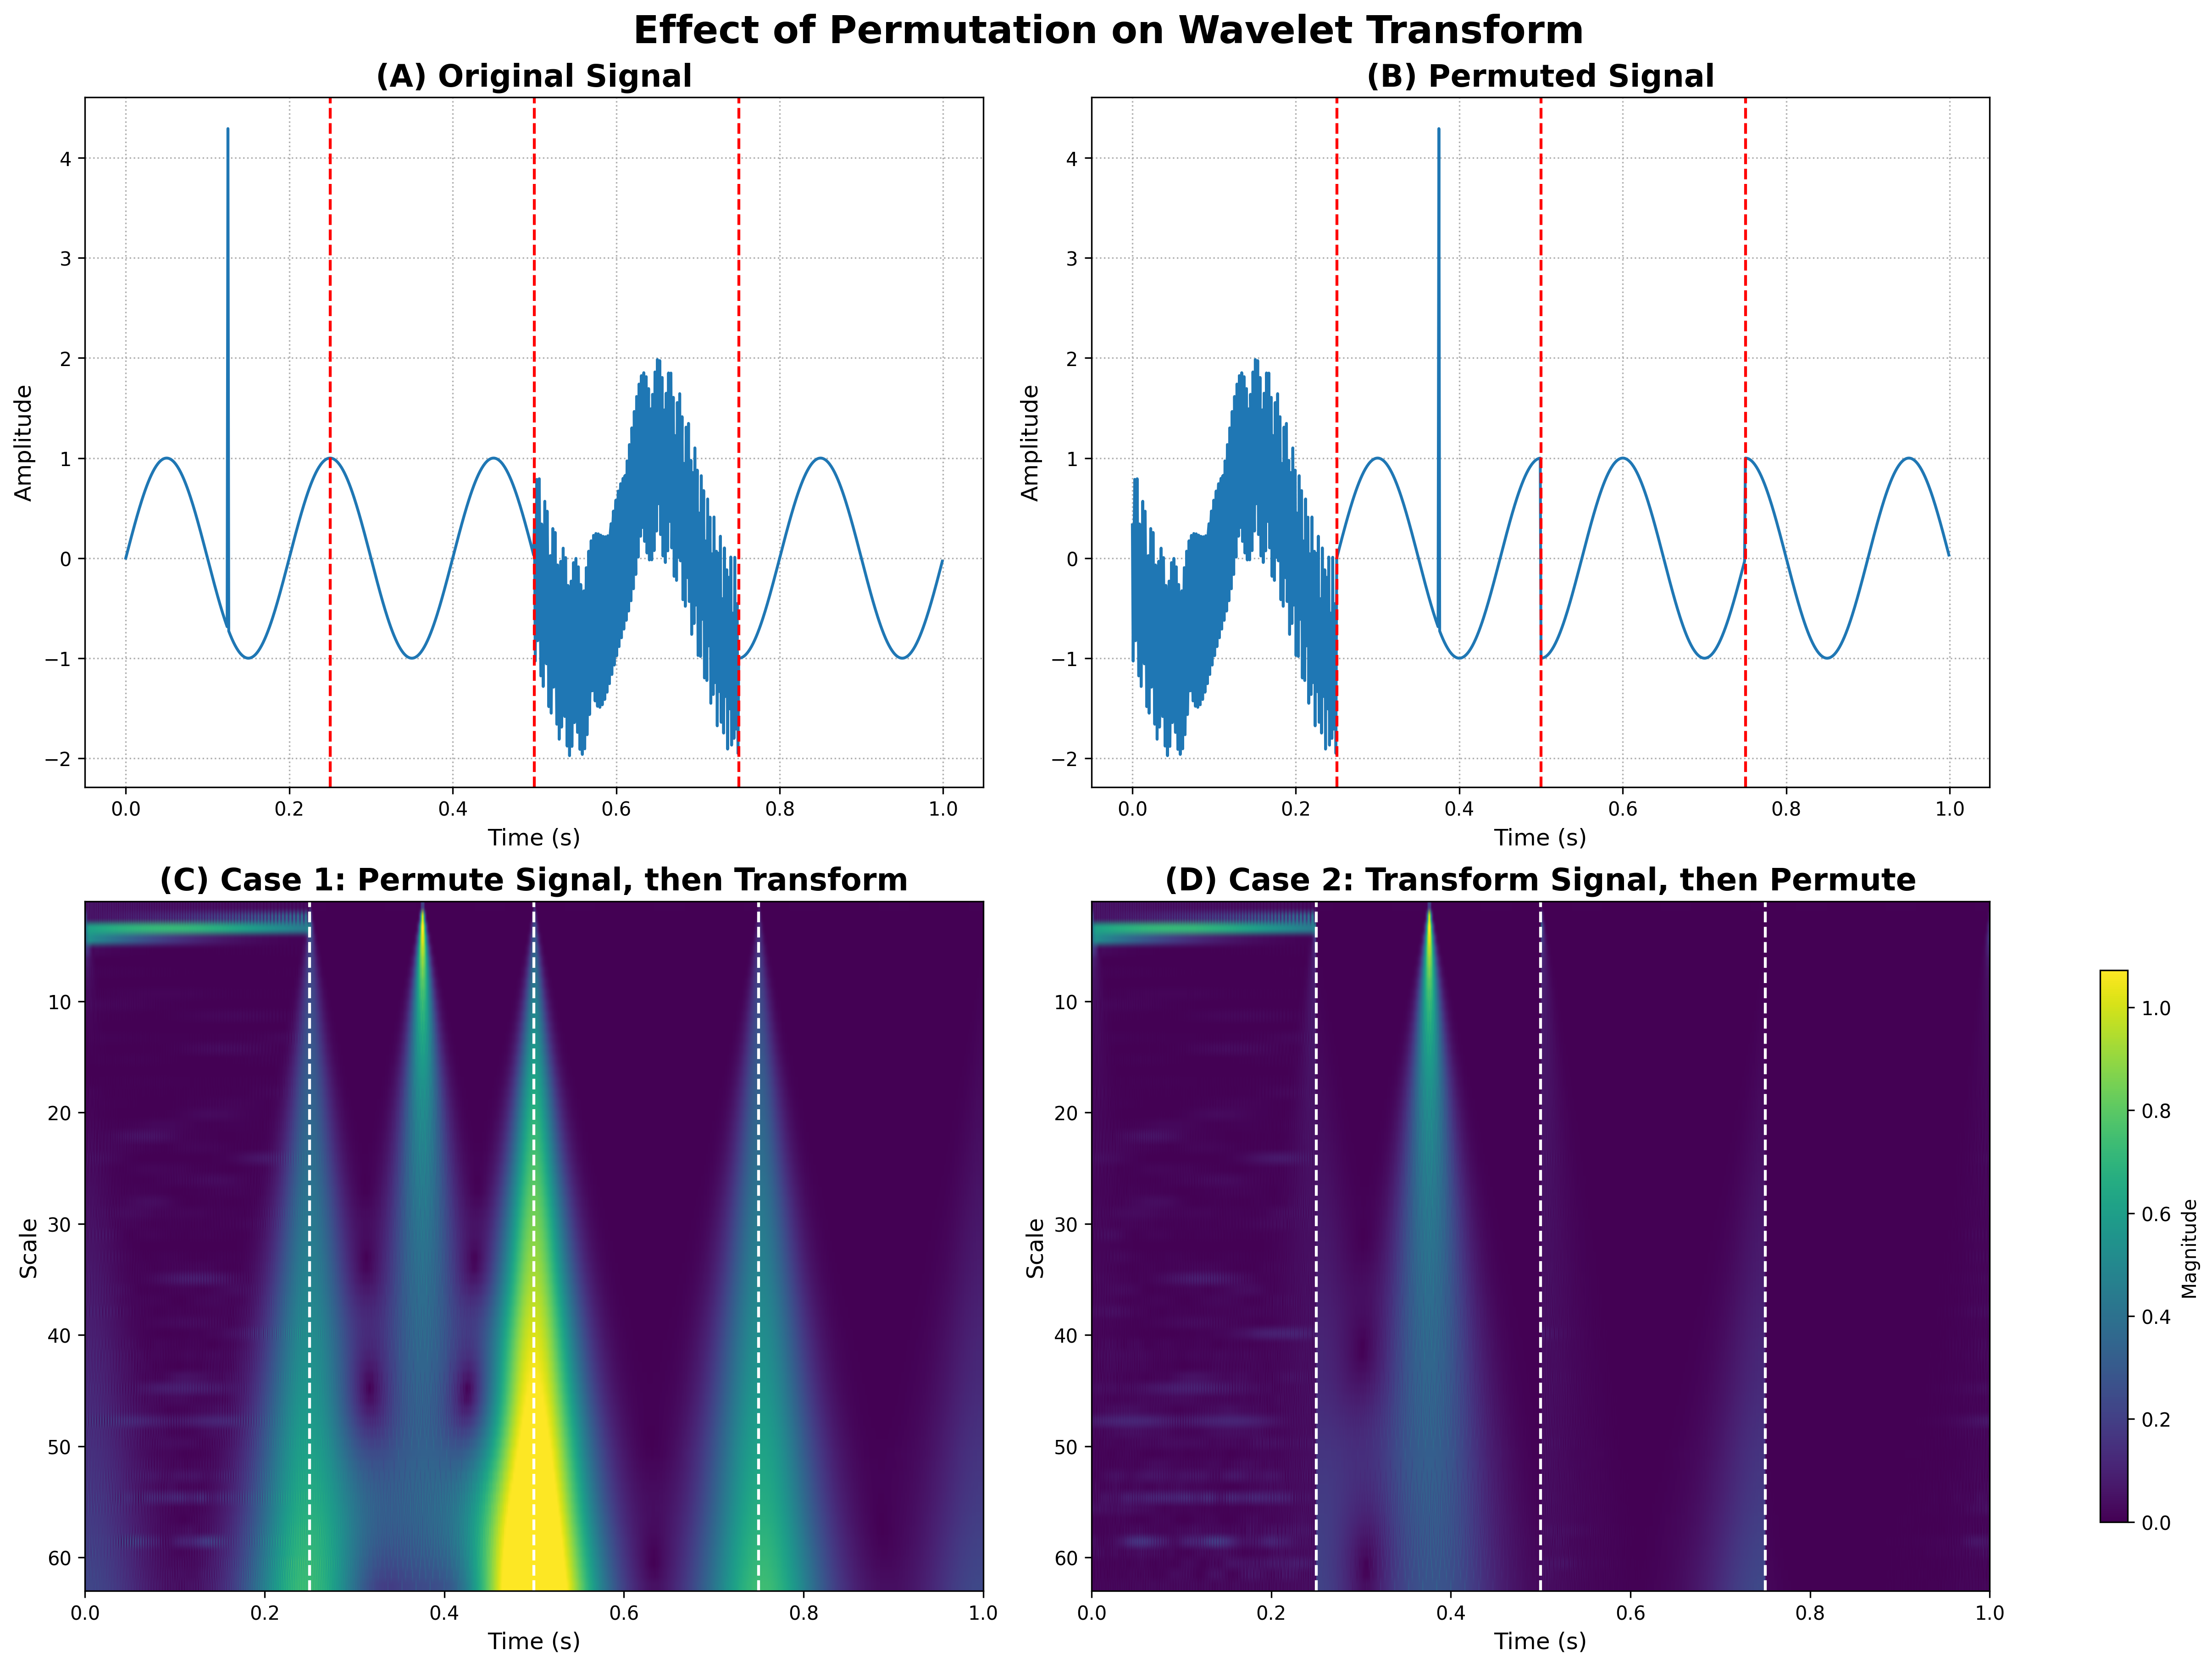
\includegraphics[width=1\textwidth]{Images/Chapter3/wavelet-permutation.png}
\caption{تاثیر ترتیب اعمال جایگشت و تبدیل موجک بر اسکالوگرام حاصل}
\label{fig:wavelet-permutation}
\end{figure}

این راهبرد یک پیش‌نیاز اساسی را به همراه دارد: تبدیلات منتخب باید به گونه‌ای باشند که ترتیب اعمال آن‌ها و تبدیل موجک، تفاوت چشمگیری در خروجی نهایی ایجاد نکند. به عبارت دیگر، نتیجه‌ی اعمال تبدیل داده‌افزایی بر روی اسکالوگرام باید تا حد امکان به نتیجه‌ی محاسبه‌ی اسکالوگرام از روی سیگنالِ داده‌افزایی‌شده نزدیک باشد. زیرا در دنیای واقعی، پدیده‌هایی مانند نویز یا چرخش حسگر، ابتدا بر سیگنال خام اثر می‌گذارند و سپس این سیگنالِ تغییریافته است که توسط ابزارهایی مانند تبدیل موجک تحلیل می‌شود.

خوشبختانه، تبدیل موجک یک تبدیل خطی است. این ویژگی ریاضی به ما اجازه می‌دهد تا تبدیلات خطی را با آن جابه‌جا کنیم بدون آنکه خروجی به شکل معناداری تغییر کند. به همین دلیل، استفاده از تبدیلات مقیاس‌دهی، معکوس‌سازی زمانی، بر زدن کانال‌ها و چرخش مشکلی ایجاد نمی‌کنند. اما نویز و جایگشت اسکالوگرام حاصل را به کلی تغییر می‌دهند. البته در رابطه با جایگشت، همانطور که در شکل \ref{fig:wavelet-permutation} قابل مشاهده است،
بخش‌های دارای فرکانس بالا (مقیاس پایین) که تغییرات محلی را در نظر می‌گیرند، تغییر چندانی ایجاد نمی‌شود اما در مقیاس‌های بالا که فرکانس‌های پایین و تغییرات سراسری را در نظر می‌گیرند، تغییرات شدیدی ایجاد می‌شود.

\section{جمع‌بندی}

در این فصل، روش پیشنهادی این پژوهش به‌طور جامع معرفی و تشریح گردید. ابتدا، معماری پایه که بر دو کدگذار مجزا برای حوزه‌های زمان و زمان-فرکانس استوار است، مورد بررسی قرار گرفت و نقاط ضعف و زمینه‌های مستعد بهبود در آن شناسایی شد. سپس، نوآوری‌های این پژوهش که برای رفع این چالش‌ها طراحی شده‌اند، ارائه گردید. نوآوری اصلی، جایگزینی چارچوب یادگیری تباینی \lr{SimCLR} با الگوریتم \lr{SwAV} بود که یک رویکرد مبتنی بر خوشه‌بندی است و با هدف یادگیری بازنمایی‌هایی پایدارتر و متمایزتر معرفی شد. علاوه بر این، راهبرد داده‌افزایی برای اسکالوگرام‌ها مورد بازنگری قرار گرفت و یک رویکرد جدید مبتنی بر تبدیلات معنادار فیزیکی که با ماهیت سیگنال‌ها سازگاری بیشتری دارد، جایگزین روش‌های پیشین شد. در فصل آتی، کارایی نوآوری‌های مطرح‌شده از طریق آزمایش‌های گسترده مورد ارزیابی قرار گرفته و نتایج حاصل از آن به تفصیل بررسی خواهد شد.
